\documentclass{amsart}
\usepackage{amsmath, amssymb}
\usepackage{tikz}
\usetikzlibrary{decorations.pathreplacing}

\title{Q\&A: Set-valued vs.\ Multiset Period}
\date{2026-05-02}

\begin{document}
\maketitle

\section*{Question}

What is the difference between the \emph{multiset} and the \emph{set} in the
context of cut-and-project sequences?

\section*{Answer}

Both objects are built from the same strip projection.  Given coprime
\(\alpha,\beta\in\mathbb{N}\) and strip parameter \(\omega\ge 0\), a lattice
point \((x,y)\in\mathbb{Z}^2\) is \emph{accepted} when it lies inside the
strip, i.e.\ when its invariant \(r = \alpha x - \beta y\) satisfies
\(r\in[-\beta\omega,\,\alpha\omega]\).  The \emph{projected value} of an
accepted point is the integer \(\tilde p = \beta x + \alpha y\) (up to a
conventional scaling).

Multiple accepted lattice points can share the same projected value \(\tilde
p\).  The two objects differ in how they handle this:

\begin{description}
  \item[Multiset.]
    Record every projected value with multiplicity.  Formally, the multiset
    assigns to each integer \(n\) a non-negative integer multiplicity
    \(\mu(n) =\) (number of accepted lattice points projecting to \(n\)).
    The \emph{multiset period} \(\lambda_{\mathrm{multiset}}\) is the minimal
    \(T>0\) such that \(\mu(n+T)=\mu(n)\) for all \(n\in\mathbb{Z}\).

  \item[Set.]
    Discard multiplicities: only ask whether each integer is present at all,
    i.e.\ whether \(\mu(n)>0\).  The \emph{set period}
    \(\lambda_{\mathrm{set}}\) is the minimal period of the binary (present /
    absent) pattern, equivalently the period of the gap sequence of the
    projected set \(S = \{n\in\mathbb{Z}: \mu(n)>0\}\).
\end{description}

\noindent
Because the set forgets multiplicities, it carries less information:
\(\lambda_{\mathrm{set}}\) always divides \(\lambda_{\mathrm{multiset}}\), and
strict inequality is possible.  Concretely:

\begin{itemize}
  \item When \(N < D\): every accepted integer has multiplicity exactly \(1\).
    The multiset and the set encode the same data, so
    \(\lambda_{\mathrm{set}} = \lambda_{\mathrm{multiset}} = N\).
  \item When \(N = D\): still multiplicity \(\le 1\), but now every integer is
    present, so the set is all of \(\mathbb{Z}\) and both periods equal \(1\).
  \item When \(N > D\): the set is again all of \(\mathbb{Z}\)
    (\(\lambda_{\mathrm{set}}=1\)), but some integers now appear with
    multiplicity \(>1\), so \(\lambda_{\mathrm{multiset}} > 1\).  The
    multiplicity sequence is non-trivial even though the set is not.
\end{itemize}

The figure in the next question illustrates all three regimes.

% -------------------------------------------------------------------
\section*{Question}

In \texttt{rational\_cut\_and\_project\_gap\_periods.tex} there is the statement:
\[
  \lambda_{\mathrm{set}} \le \lambda_{\mathrm{multiset}}
  \quad\text{in every case, with equality if and only if } N \le D.
\]
The case \(N < D\) is clear.  What about \(N = D\)?

\section*{Answer}

The proof handles the three sub-regimes in the corollary (Corollary~6.2 in the
paper):

\begin{description}
  \item[\(N < D\).]
    The multiplicity function \(\mu\) takes values in \(\{0,1\}\): exactly
    \(N\) residue classes are hit once, the remaining \(D - N\) are hit zero
    times.  No integer has multiplicity greater than one, so the underlying
    \emph{set} coincides with the multiset as sequences, and
    \(\lambda_{\mathrm{set}} = \lambda_{\mathrm{multiset}} = N\).
    Equality holds because the two objects are genuinely the same.

  \item[\(N = D\).]
    Since \(D \mid N\) (trivially, \(N/D = 1\)), Theorem~3.1 gives
    \(\lambda_{\mathrm{multiset}} = N/D = 1\).  Simultaneously, the condition
    \(N \ge D\) means every residue class mod \(D\) is hit by the projected
    sequence; when \(N = D\) exactly, each class is hit exactly once (no
    over-representation).  Hence every integer appears in the projected set,
    the gap sequence is constantly \(1\), and \(\lambda_{\mathrm{set}} = 1\).
    Both periods equal \(1\) and equality holds, but for a \emph{degenerate}
    reason: the sequence is trivially periodic because the set is all of
    \(\mathbb{Z}\) and the multiset is uniform with multiplicity \(1\).

  \item[\(N > D\).]
    Again every residue class is hit (multiplicity \(\ge 1\) everywhere), so
    \(\lambda_{\mathrm{set}} = 1\).  But now \(\lambda_{\mathrm{multiset}} > 1\)
    (it equals \(N/D \ge 2\) when \(D \mid N\), and \(N \ge 2\) when
    \(D \nmid N\)), giving \emph{strict} inequality.
\end{description}

\medskip\noindent
In summary: equality \(\lambda_{\mathrm{set}} = \lambda_{\mathrm{multiset}}\)
holds for \(N \le D\), covering both the non-degenerate case (\(N < D\), where
the set and multiset genuinely agree) and the degenerate boundary case
(\(N = D\), where both periods collapse to~\(1\)).

% -------------------------------------------------------------------
\section*{Question}

What is the geometric meaning of \(N\) and \(D\) in
\[
  N \;:=\; \lfloor\omega\alpha\rfloor + \lfloor\omega\beta\rfloor + 1,
  \qquad
  D \;:=\; \alpha^2 + \beta^2\,?
\]

\section*{Answer}

\paragraph{The invariant \(r = \alpha x - \beta y\).}
Given a lattice point \((x,y)\in\mathbb{Z}^2\), the value \(r = \alpha x - \beta y\)
is constant along each line parallel to the projection direction \(f(x)=(\alpha/\beta)x\).
One can therefore label every accepted lattice point by its invariant \(r\).
Feasibility of the cut imposes \(r \in [-\beta\omega,\,\alpha\omega]\), and
\(N\) is precisely the number of integers in this closed interval:
\[
  N \;=\; \#\bigl(\mathbb{Z}\cap[-\beta\omega,\,\alpha\omega]\bigr)
    \;=\; \lfloor\omega\alpha\rfloor + \lfloor\omega\beta\rfloor + 1.
\]
For example, with \(\alpha=2\), \(\beta=1\) (the running example of Figure~\ref{fig:residue}):
\begin{itemize}
  \item \(\omega = 1\): interval \([-1,\,2]\),
    integers \(\{-1,0,1,2\}\),
    \(N = \lfloor 2\rfloor + \lfloor 1\rfloor + 1 = 2+1+1 = 4\).
  \item \(\omega = \tfrac{3}{2}\): interval \([-\tfrac{3}{2},\,3]\),
    integers \(\{-1,0,1,2,3\}\),
    \(N = \lfloor 3\rfloor + \lfloor \tfrac{3}{2}\rfloor + 1 = 3+1+1 = 5\).
  \item \(\omega = 2\): interval \([-2,\,4]\),
    integers \(\{-2,-1,0,1,2,3,4\}\),
    \(N = \lfloor 4\rfloor + \lfloor 2\rfloor + 1 = 4+2+1 = 7\).
\end{itemize}
These are exactly the three values of \(N\) shown in Figure~\ref{fig:residue}.

A further example showing the general structure:
if \(\omega\alpha = 3.7\) and \(\omega\beta = 3.5\), then
\(\lfloor\omega\alpha\rfloor = 3\), \(\lfloor\omega\beta\rfloor = 3\), and
\(N = 3 + 3 + 1 = 7\).
The interval \([-3.5,\,3.7]\) contains exactly the seven integers
\(-3,-2,-1,0,1,2,3\), labelled \(1\) through \(7\) (track indices) in the
diagram below.

\begin{center}
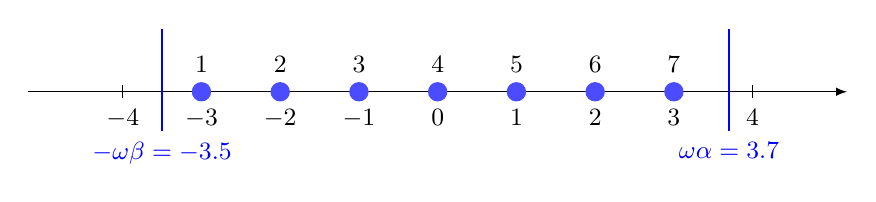
\begin{tikzpicture}[>=latex, scale=1.0]
  % Number line
  \draw[->] (-5.2, 0) -- (5.2, 0);

  % Tick marks and lower labels (integers -4 .. 4)
  \foreach \n in {-4,...,4} {
    \draw (\n, 0.08) -- (\n, -0.08);
    \node[below, font=\small] at (\n, -0.10) {$\n$};
  }

  % Interval boundary lines
  \draw[thick, blue] (-3.5, -0.5) -- (-3.5,  0.8);
  \draw[thick, blue] ( 3.7, -0.5) -- ( 3.7,  0.8);

  % Boundary labels
  \node[below, font=\small, blue] at (-3.5, -0.52)
    {$-\omega\beta = -3.5$};
  \node[below, font=\small, blue] at ( 3.7, -0.52)
    {$\omega\alpha = 3.7$};

  % Highlight the 7 integers inside the interval
  \foreach \n in {-3,...,3} {
    \fill[blue!70] (\n, 0) circle (3.5pt);
  }

  % Track-index labels above (1 .. 7)
  \foreach \n/\k in {-3/1, -2/2, -1/3, 0/4, 1/5, 2/6, 3/7} {
    \node[above, font=\small] at (\n, 0.12) {$\k$};
  }
\end{tikzpicture}
\end{center}

\noindent
The count gives \(N = \lfloor 3.7\rfloor + \lfloor 3.5\rfloor + 1 = 3+3+1 = 7\).

Geometrically, each admissible value of \(r\) indexes one \emph{track}: the
set of projected values \(\tilde{p}\) coming from lattice points with that
particular invariant.

\paragraph{Why \(D = \alpha^2+\beta^2\) is the common difference.}
Projected onto the \(\tilde{p}\)-axis, the lattice points on a single track
form an arithmetic progression.  Moving one step along the track --- i.e.\
incrementing \(x\) by \(\beta\) and \(y\) by \(\alpha\) to keep \(r\) constant
--- changes the projected value \(\tilde{p}\) by
\[
  \Delta\tilde{p}
  \;=\; \beta\cdot\beta + \alpha\cdot\alpha
  \;=\; \alpha^2+\beta^2 \;=\; D.
\]
Thus every track is an arithmetic progression with common difference \(D\),
and \(D = \|(\beta,\alpha)\|^2\) is also the squared length of the direction
vector of \(f\).

\paragraph{Role in the period formula.}
The \(N\) tracks produce \(N\) residue classes modulo \(D\), one per track.
The map \(r \mapsto c_r \bmod D\) (where \(c_r \equiv -\alpha\beta^{-1}r\)) is
multiplication by a unit, hence a bijection on \(\mathbb{Z}/D\mathbb{Z}\).
As \(r\) runs over \(N\) consecutive integers:
\begin{itemize}
  \item If \(N < D\): not all \(D\) residue classes are reached.  Some integers
        are never a projected value, so the integer line has periodic gaps
        and the period is \(N\).
  \item If \(N = D\): exactly one full cycle is completed.  Every residue class
        is hit once, every integer appears, and both periods equal \(1\).
  \item If \(N > D\): more than one full cycle, so every residue class is
        hit at least once (some more than once).  The set-valued period is
        \(1\), but the multiset period reflects the non-uniform multiplicity
        distribution and equals \(N\) (if \(D \nmid N\)) or \(N/D\)
        (if \(D \mid N\)).
\end{itemize}
Figure~\ref{fig:residue} illustrates all three regimes for
\(\alpha=2\), \(\beta=1\), \(D=5\).

\begin{figure}[ht]
\centering
\resizebox{\linewidth}{!}{%
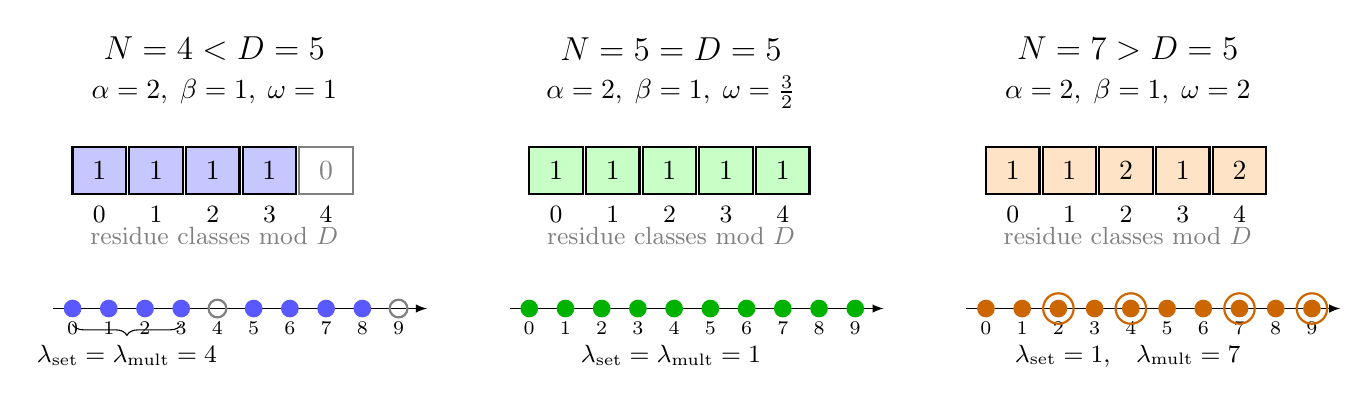
\begin{tikzpicture}[>=latex]

% Layout constants
\def\bw{0.68}   % box width
\def\bh{0.60}   % box height
\def\bs{0.04}   % gap between boxes
\def\step{0.72} % box pitch  (\bw + \bs rounded up)
\def\ns{0.46}   % integer spacing on number line

%% ---- CASE A: N=4 < D=5, omega=1 -------------------------
\begin{scope}[xshift=0cm]
  \node[font=\large\bfseries, align=center] at (1.80,5.6)
    {$N=4 < D=5$};
  \node[font=\normalsize] at (1.80,5.05)
    {$\alpha=2,\;\beta=1,\;\omega=1$};

  % Residue-class boxes (classes 0..4, multiplicities 1,1,1,1,0)
  % Class labels below
  \foreach \i in {0,...,4} {
    \node[font=\small] at (\i*\step+0.34, 3.50) {$\i$};
  }
  % Fill covered classes (0,1,2,3) in blue, leave class 4 empty
  \foreach \i in {0,...,3} {
    \fill[blue!22] (\i*\step, 3.75) rectangle (\i*\step+\bw, 3.75+\bh);
    \draw[thick]   (\i*\step, 3.75) rectangle (\i*\step+\bw, 3.75+\bh);
    \node[font=\normalsize] at (\i*\step+0.34, 4.05) {$1$};
  }
  \draw[thick, gray] (4*\step, 3.75) rectangle (4*\step+\bw, 3.75+\bh);
  \node[font=\normalsize,gray] at (4*\step+0.34, 4.05) {$0$};

  \node[font=\small,gray] at (1.80, 3.22) {residue classes mod $D$};

  % Number line: integers 0..9 (two full periods)
  \draw[->] (-0.25, 2.30) -- (4.50, 2.30);
  % Present: all except those ≡ 4 mod 5 (i.e., 4 and 9)
  \foreach \n in {0,1,2,3,5,6,7,8} {
    \fill[blue!65] (\n*\ns, 2.30) circle (3.2pt);
  }
  \foreach \n in {4,9} {
    \draw[gray, thick] (\n*\ns, 2.30) circle (3.2pt);
  }
  \foreach \n in {0,...,9} {
    \node[below, font=\scriptsize] at (\n*\ns, 2.25) {$\n$};
  }

  % Brace over one period (elements 0,1,2,3 → 4 dots)
  \draw[decorate,decoration={brace,amplitude=4pt,mirror,raise=4pt}]
    (0, 2.24) -- (3*\ns, 2.24);
  \node[font=\small] at (1.5*\ns, 1.70)
    {$\lambda_{\mathrm{set}}=\lambda_{\mathrm{mult}}=4$};
\end{scope}

%% ---- CASE B: N=5 = D=5, omega=3/2 -------------------------
\begin{scope}[xshift=5.8cm]
  \node[font=\large\bfseries, align=center] at (1.80,5.6)
    {$N=5 = D=5$};
  \node[font=\normalsize] at (1.80,5.05)
    {$\alpha=2,\;\beta=1,\;\omega=\tfrac{3}{2}$};

  \foreach \i in {0,...,4} {
    \fill[green!22] (\i*\step, 3.75) rectangle (\i*\step+\bw, 3.75+\bh);
    \draw[thick]    (\i*\step, 3.75) rectangle (\i*\step+\bw, 3.75+\bh);
    \node[font=\small] at (\i*\step+0.34, 3.50) {$\i$};
    \node[font=\normalsize] at (\i*\step+0.34, 4.05) {$1$};
  }
  \node[font=\small,gray] at (1.80, 3.22) {residue classes mod $D$};

  \draw[->] (-0.25, 2.30) -- (4.50, 2.30);
  \foreach \n in {0,...,9} {
    \fill[green!70!black] (\n*\ns, 2.30) circle (3.2pt);
    \node[below, font=\scriptsize] at (\n*\ns, 2.25) {$\n$};
  }
  \node[font=\small] at (1.80, 1.70)
    {$\lambda_{\mathrm{set}}=\lambda_{\mathrm{mult}}=1$};
\end{scope}

%% ---- CASE C: N=7 > D=5, omega=2 -------------------------
\begin{scope}[xshift=11.6cm]
  \node[font=\large\bfseries, align=center] at (1.80,5.6)
    {$N=7 > D=5$};
  \node[font=\normalsize] at (1.80,5.05)
    {$\alpha=2,\;\beta=1,\;\omega=2$};

  % Multiplicities: 0→1, 1→1, 2→2, 3→1, 4→2
  \foreach \i/\m in {0/1, 1/1, 2/2, 3/1, 4/2} {
    \fill[orange!22] (\i*\step, 3.75) rectangle (\i*\step+\bw, 3.75+\bh);
    \draw[thick]     (\i*\step, 3.75) rectangle (\i*\step+\bw, 3.75+\bh);
    \node[font=\small] at (\i*\step+0.34, 3.50) {$\i$};
    \node[font=\normalsize\bfseries] at (\i*\step+0.34, 4.05) {$\m$};
  }
  \node[font=\small,gray] at (1.80, 3.22) {residue classes mod $D$};

  % All integers present; ring doubled positions (≡2 and ≡4 mod 5)
  \draw[->] (-0.25, 2.30) -- (4.50, 2.30);
  \foreach \n in {0,...,9} {
    \fill[orange!80!black] (\n*\ns, 2.30) circle (3.2pt);
    \node[below, font=\scriptsize] at (\n*\ns, 2.25) {$\n$};
  }
  % Extra ring at doubled positions: 2,4,7,9
  \foreach \n in {2,4,7,9} {
    \draw[orange!80!black, thick] (\n*\ns, 2.30) circle (5.5pt);
  }

  \node[font=\small, align=center] at (1.80, 1.70)
    {$\lambda_{\mathrm{set}}=1$,\quad
     $\lambda_{\mathrm{mult}}=7$};
\end{scope}

\end{tikzpicture}
}% end resizebox
\caption{Residue-class coverage for $\alpha=2$, $\beta=1$, $D=\alpha^2+\beta^2=5$.
  The numbers in each box show the multiplicity (how many of the $N$ tracks cover
  that residue class).
  Filled dots on the number line indicate integers present in the projected set;
  open circles mark absent integers.
  Ringed dots (right panel) mark integers that appear with multiplicity $>1$ in the
  multiset.
  \emph{Left:} One residue class is empty; one integer in every five is missing,
  giving gap pattern $(1,1,1,2)$ with period $N=4$.
  \emph{Centre:} All classes covered with multiplicity exactly $1$; every integer
  appears, both periods equal $1$.
  \emph{Right:} All classes covered, some with multiplicity $2$; the set still
  contains every integer ($\lambda_{\mathrm{set}}=1$), but the multiset carries
  non-uniform multiplicities, yielding gap pattern $(1,1,0,1,1,0,1)$ with
  $\lambda_{\mathrm{mult}}=N=7$.}
\label{fig:residue}
\end{figure}

% -------------------------------------------------------------------
\section*{Question}

The paper says: ``the set-valued period collapses to \(1\) because every
integer residue class is then hit'' (when \(N \ge D\)).  What does this mean?

\section*{Answer}

\paragraph{How each track covers one residue class.}
For each admissible invariant value \(r\), the projected values from track~\(r\)
form the arithmetic progression
\[
  P_r \;=\; \{c_r + kD : k \in \mathbb{Z}\},
  \qquad c_r \equiv -\alpha\beta^{-1}r \pmod{D}.
\]
Every integer in \(P_r\) belongs to the same residue class \(c_r \bmod D\).
To say that residue class \(c_r\) is ``hit'' means that there exists a track
whose projected values have remainder \(c_r\) when divided by \(D\).

\paragraph{Why \(N \ge D\) forces all residue classes to be hit.}
As \(r\) ranges over the \(N\) admissible values (consecutive integers), the
map \(r \mapsto c_r \bmod D\) cycles through all \(D\) residue classes
periodically, because it is multiplication by the unit \(-\alpha\beta^{-1}\)
modulo \(D\) (Corollary~6.1 of the paper ensures this is indeed a bijection on
\(\mathbb{Z}/D\mathbb{Z}\)).  After \(D\) steps every class has been hit once;
after \(2D\) steps, twice; and so on.  If \(N \ge D\), there is at least one
complete cycle, so every residue class modulo \(D\) appears among the \(N\)
classes \(\{c_r \bmod D\}\).

\paragraph{Why this forces \(\lambda_{\mathrm{set}} = 1\).}
Because every residue class \(c \in \mathbb{Z}/D\mathbb{Z}\) is hit by at
least one track, the union \(S = \bigcup_r P_r\) contains at least one element
from each class.  But each \(P_r\) already contains \emph{all} integers in
class \(c_r\) (the full AP \(c_r + kD\) for \(k\in\mathbb{Z}\)).  Hence every
integer belongs to \(S\): the projected set is all of \(\mathbb{Z}\).  A set
equal to \(\mathbb{Z}\) has gap sequence constantly \(1\), which is periodic
with minimal period \(\lambda_{\mathrm{set}} = 1\).

\paragraph{Summary.}
\(N \ge D\) means the \(N\) tracks cover all \(D\) residue classes mod \(D\).
That in turn means the set of projected values is all of \(\mathbb{Z}\), so
there are no gaps at all and the set-valued period is trivially \(1\).

% -------------------------------------------------------------------
\section*{Question}

Can you walk through the proof that \(\lambda_{\mathrm{multiset}} = N\) (for the
case \(N < D\)) step by step, using analogies from engineering?

\section*{Answer}

The proof rests on three number-theoretic tools and then proceeds in five
steps.  The engineering analogies below use gear wheels throughout.

\subsection*{Key mathematical tools}

\begin{enumerate}

  \item \textbf{Modular arithmetic (\(x \equiv y \pmod{D}\)).}
    Two integers are \emph{equal modulo \(D\)} if they leave the same remainder
    when divided by \(D\) --- ``clock arithmetic.''\\
    \textit{Engineering analogy.}  Imagine a gear with \(D\) teeth numbered
    \(0\) to \(D-1\).  Rotating the gear by \(x\) teeth lands on the same
    tooth as rotating it by \(y\) teeth exactly when \(x \equiv y \pmod{D}\).

  \item \textbf{Coprimality (\(\gcd(a,b)=1\)).}
    Two integers are \emph{coprime} if their greatest common divisor is \(1\),
    i.e.\ they share no common factor.\\
    \textit{Engineering analogy.}  If a pinion with \(a\) teeth drives a wheel
    with \(b\) teeth and \(\gcd(a,b)=1\), then over time \emph{every} tooth of
    the pinion meets \emph{every} tooth of the wheel --- no localised wear.

  \item \textbf{Modular inverse (\(a^{-1} \pmod{D}\)).}
    In ordinary arithmetic the inverse of \(3\) is \(1/3\).  In modular
    arithmetic (integers only) the inverse of \(a\) is an integer \(x\) such
    that \(a \cdot x \equiv 1 \pmod{D}\).  Such an \(x\) exists \textbf{if and
    only if} \(\gcd(a,D)=1\).

    \begin{itemize}
      \item \textit{Example (inverse exists).}  Find \(3^{-1} \pmod{7}\).
        Testing: \(3\cdot1\equiv3\), \(3\cdot2\equiv6\), \(3\cdot3\equiv2\),
        \(3\cdot4\equiv5\), \(\mathbf{3\cdot5=15\equiv1\pmod{7}}\).
        So \(5\) is the modular inverse of \(3\) modulo \(7\).

      \item \textit{Example (inverse does not exist).}  Find \(2^{-1}\pmod{4}\).
        Testing: \(2\cdot1\equiv2\), \(2\cdot2\equiv0\), \(2\cdot3\equiv2\),
        \(2\cdot4\equiv0\pmod{4}\).  Since \(\gcd(2,4)=2\neq1\), the remainder
        \(1\) is never reached and no inverse exists.

      \item \textit{Engineering analogy.}  If a pinion with \(a\) teeth drives a
        wheel with \(D\) teeth and \(\gcd(a,D)=1\), there is exactly one number
        of pinion revolutions \(x\) after which the large wheel has advanced by
        \emph{exactly one tooth} from its starting position.  That count \(x\)
        is the modular inverse.
    \end{itemize}

\end{enumerate}

\subsection*{Step 1 --- The invariant \(r\) (the ``tracks'')}

The strip is defined by
\[
  -\beta\omega \;\le\; \alpha x - \beta y \;\le\; \alpha\omega.
\]
The expression \(r := \alpha x - \beta y\) is an \emph{invariant}: it is
constant along every line parallel to the projection direction \((\beta,\alpha)\).
Moving one lattice step in that direction --- from \((x,y)\) to
\((x+\beta,\,y+\alpha)\) --- leaves \(r\) unchanged:
\[
  \alpha(x+\beta)-\beta(y+\alpha)=\alpha x+\alpha\beta-\beta y-\beta\alpha
  =\alpha x-\beta y=r.
\]
Each integer value of \(r\) in \([-\beta\omega,\alpha\omega]\) therefore
represents a continuous \emph{track} of lattice points.  The number of such
integers is exactly \(N\), so there are \(N\) tracks.

\subsection*{Step 2 --- The linear system}

For a fixed track \(r\) we want to know which projected positions \(\tilde{p}\)
are visited.  The projected value is \(\tilde{p}=\beta x+\alpha y\).  Together
with the track condition this gives a \(2\times2\) system:
\begin{align*}
  \beta x + \alpha y &= \tilde{p},\\
  \alpha x - \beta y &= r.
\end{align*}
The determinant is \(-\alpha^2-\beta^2=-D\), so the solution is
\[
  x = \frac{\beta\tilde{p}+\alpha r}{D}, \qquad
  y = \frac{\alpha\tilde{p}-\beta r}{D}.
\]
For \((x,y)\) to be a lattice point both values must be integers, which requires
\(D \mid \beta\tilde{p}+\alpha r\), i.e.\
\[
  \beta\tilde{p} \equiv -\alpha r \pmod{D}.
\]
Multiplying both sides by \(\beta^{-1}\) (justified in Step~3):
\[
  \tilde{p} \equiv -\alpha\beta^{-1}r \pmod{D}.
\]
\textbf{Conclusion.}  On track \(r\), projected values do not occur at every
integer, but only at positions belonging to the residue class
\(c_r := -\alpha\beta^{-1}r \bmod D\).  Each track thus produces an arithmetic
progression with common difference \(D\) and offset \(c_r\).

\subsection*{Step 3 --- Coprimality of \(\beta\) and \(D\)}

The step above used \(\beta^{-1}\pmod{D}\).  This exists because
\(\gcd(\beta,D)=1\).  Indeed, \(D=\alpha^2+\beta^2\), and since
\(\gcd(\alpha,\beta)=1\) (a standing assumption), \(\beta\) can share no common
factor with \(\alpha^2+\beta^2\) other than \(1\).  Hence \(\beta^{-1}\pmod{D}\)
always exists.

\subsection*{Step 4 --- Distribution of tracks around the gear}

We have \(N\) tracks with consecutive integer values of \(r\).  Each track
contributes a residue class \(c_r\) that advances by the fixed step
\(m:=-\alpha\beta^{-1}\bmod D\) each time \(r\) increases by \(1\).  Since
\(\gcd(m,D)=1\) (again by coprimality), the gear analogy applies: stepping
through all \(N\) tracks visits residue classes in a pattern that cycles through
\emph{every} residue class before repeating --- a bijection on
\(\mathbb{Z}/D\mathbb{Z}\).

Writing \(N = q\cdot D + s\) (\(0 \le s < D\)):
\begin{itemize}
  \item \(s\) residue classes are hit \(q+1\) times (``heavy'' teeth),
  \item the remaining \(D-s\) classes are hit \(q\) times.
\end{itemize}
Crucially, because the steps \(r, r+1, r+2,\dots\) are consecutive, the
\(s\) heavy classes form a \textbf{contiguous block} (a cyclic interval) around
the gear.

\subsection*{Step 5 --- Minimality (proof by contradiction)}

Suppose the gap pattern had a period \(\lambda' < N\).  Since \(N\) is itself a
period, \(\lambda'\) would have to divide \(N\).  A period \(\lambda'\) means
that shifting the entire projected pattern by some distance \(\sigma\)
(corresponding to \(\lambda'\) consecutive gaps) maps it identically onto itself.

Shifting the pattern is equivalent to rotating the residue-class gear by
\(\sigma \bmod D\).  For the pattern to look identical after the rotation, the
heavy classes must land back on heavy classes.  But the heavy classes form a
\emph{single contiguous arc} on the gear.

A contiguous arc on a circle can only map onto itself under a rotation that is
either \(0\) (no rotation) or a full \(360^\circ\) (one complete turn).
Analogously: if you mark a connected block of, say, \(3\) out of \(8\) cake
slices, the only rotation that puts those \(3\) slices exactly back on
themselves is a full turn.

The only rotation of the gear that returns the arc to itself is therefore a
multiple of \(D\), which corresponds to a shift of exactly \(N\) points --- not
any smaller \(\lambda'\).

\textbf{Conclusion.}  No period smaller than \(N\) can exist.  The multiset
period is therefore minimal at \(\lambda_{\mathrm{multiset}} = N\). \qed

\end{document}
